\documentclass{article}
\usepackage{graphicx}
\usepackage{amsmath}
\usepackage{hyperref}
\usepackage{siunitx}

\usepackage{pgfplots}
\usepackage{filecontents}

\graphicspath{ {./images/} }

%-------------------------------------------------------------------------------
%	TITLE SECTION
%-------------------------------------------------------------------------------

\newcommand{\horrule}[1]{\rule{\linewidth}{#1}} % Create horizontal rule command with 1 argument of height

\title{
\normalfont \normalsize
\textsc{Sapienza University of Rome} \\ [25pt] % Your university, school and/or department name(s)
\horrule{0.5pt} \\[0.4cm] % Thin top horizontal rule
\LARGE Atom Simulator \\ % The assignment title
\large Interactive Graphics \\
\horrule{2pt} \\[0.5cm] % Thick bottom horizontal rule
}

\author{Ibis Prevedello} % Your name

\date{\normalsize\today} % Today's date or a custom date

\begin{document}
\sloppy % avoid to make words to go out of margin

\maketitle % Print the title

%-------------------------------------------------------------------------------

\section{Introduction}

The goal of this project is to create an atom simulator, where the user can see and interact with any element of the periodic table, with its correct number of protons, neutrons and electrons. Also, for any element chosen, it also presents its relevant information, as shown in figure \ref{fig:fig5}. The idea is to develop a fun and easy platform that can be used by students while learning chemistry, once that what are usually shown during classes are very poor 2D drawings.

This project was developed using three.js, which is a cross-browser JavaScript library and Application Programming Interface (API) used to create and display animated 3D computer graphics in a web browser and uses WebGL.

The source code of this project can be found on \href{https://github.com/ibiscp/Atom-Simulator}{GitHub} and it can be tested in \href{https://ibiscp.000webhostapp.com/atom.html}{this link}. The project was also sent to \href{https://experiments.withgoogle.com/}{Experiments with Google} and is still under evaluation.

\begin{figure}[!ht]
\centering
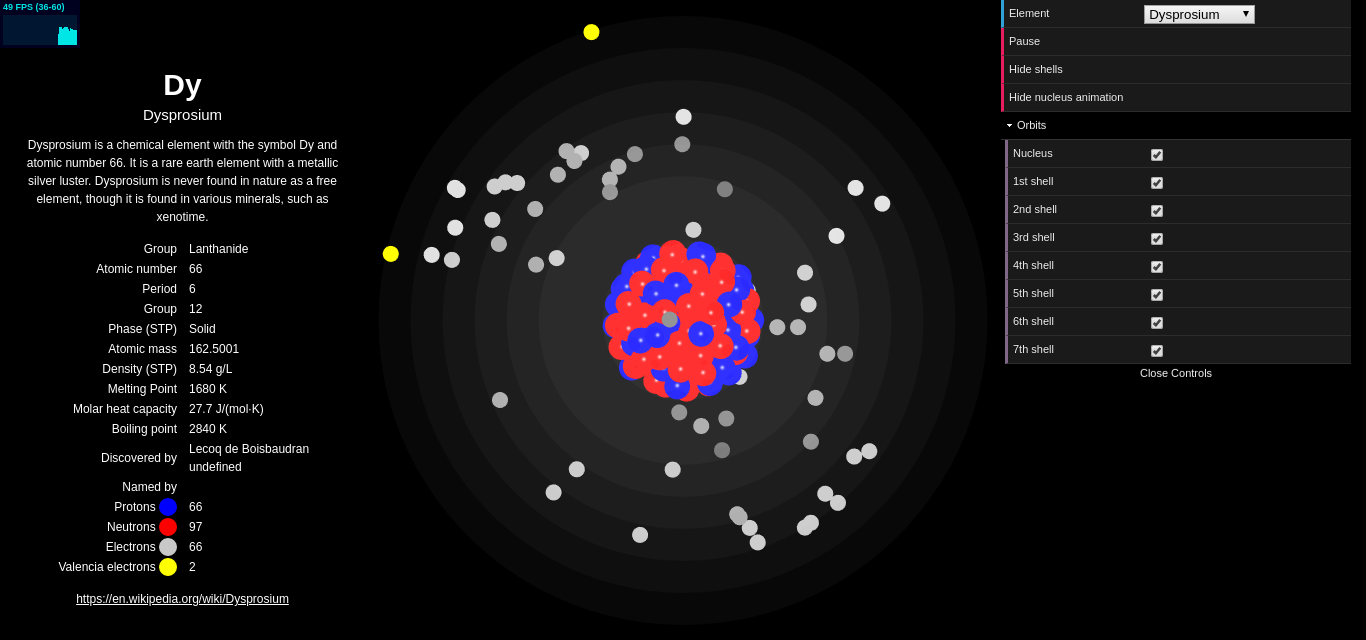
\includegraphics[scale=0.25]{screenshot.png}
\caption{Atom simulator running}
\label{fig:fig5}
\end{figure}

%-------------------------------------------------------------------------------

\section{Hierarchical Model}

The model implemented is not complicated and thus the hierarchical model is simple. The model elements are basically all centered at the origin, with exception of protons and neutrons that are translated inside the nucleus.

Below is presented the hierarchy used, the vector of shells is taken as parent and the rest of the elements taken as children.

\begin{itemize}
	\item Shells
		\begin{itemize}
			\item Nucleus Elements
			\begin{itemize}
				\item Protons
				\item Neutrons
			\end{itemize}
			\item Electrons
		\end{itemize}
\end{itemize}

%-------------------------------------------------------------------------------

\section{Implementation}

Below is presented in detail all the features developed for the project, including the nucleus generation, electron orbits, user controls and information card.

\subsection{Nucleus generation}

This was by far the most difficult task of the project, at the end the solution achieved was really simple, however the process was very challenging. There is not a formula or a simple algorithm to position \textit{n} spheres with a maximum radius inside another sphere with a fixed radius \textit{R} without overlapping.

This problem is known as 'sphere packing problem' and there are some recursive algorithms to achieve the best result, however, because this was not the main focus of the project and something more easy and straight forward was needed, it was decided to implement a simpler version of the sphere packing algorithm.

The implementation chosen does not achieve a perfect arrangement and the spheres end up overlapping a little bit of the edges. For this implementation the internal spheres start with a radius equivalent to fill 1\% of the total volume of the container and increase its radius continuously and rearrange itself, avoiding overlapping with each other and with the container till a point where the overlapping achieves a maximum threshold, this process is presented in figure \ref{fig:fig1}.

Also, while they are expanding, they are also doing random walk in order to achieve the rearrangement.

\begin{figure}[!ht]
\centering
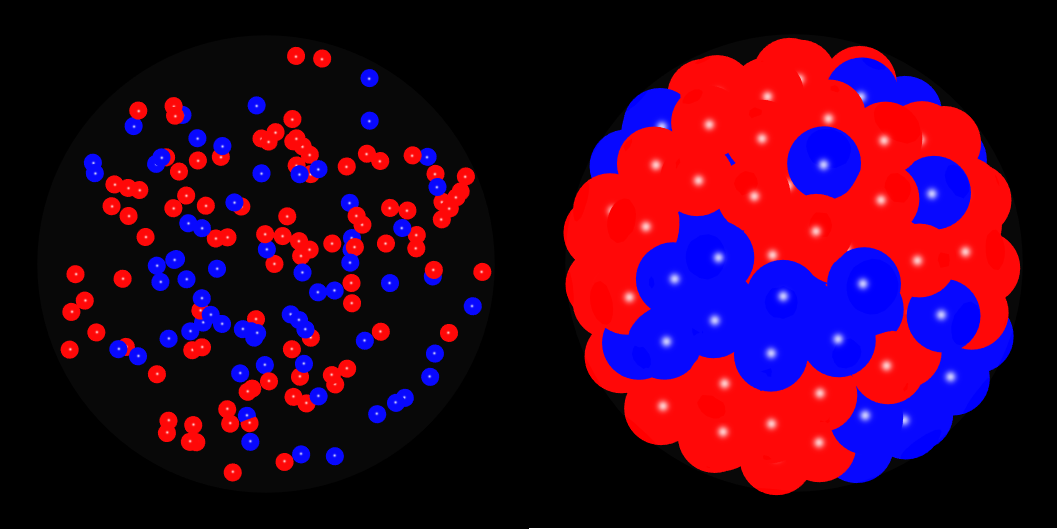
\includegraphics[scale=0.3]{nucleus_formation.png}
\caption{Before and after of nucleus generation process}
\label{fig:fig1}
\end{figure}

\subsection{Electron orbits}

The electrons are placed in its correct orbit obeying the electron configuration, presented in figure \ref{fig:fig2}. The color and the speed are also changing gradually as the orbit is expanding.

\begin{figure}[!ht]
\centering
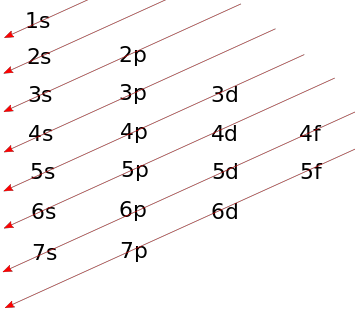
\includegraphics[scale=0.4]{electron_configuration.png}
\caption{Electron configuration}
\label{fig:fig2}
\end{figure}

For the last layer, the electrons are colored yellow, to show that these are the valence electrons, which are electrons in one of the outer shells of an atom that can participate in forming chemical bonds with other atoms (figure \ref{fig:fig3}).

\begin{figure}[!ht]
\centering
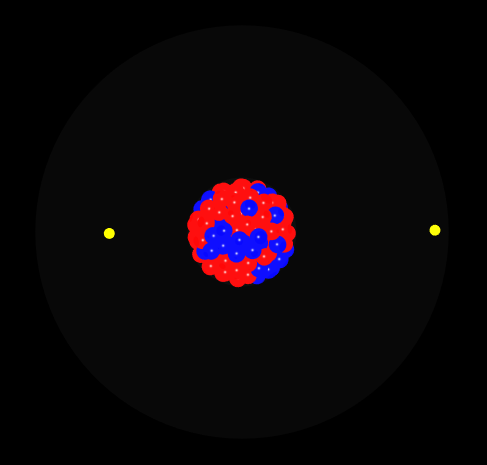
\includegraphics[scale=0.4]{valence_electrons.png}
\caption{Valence electrons}
\label{fig:fig3}
\end{figure}

\subsection{User controls}

The controls represent one way for the user to interact with the simulation, with the controls one can chose the element to be simulated, pause and continue animation, show or hide the shells, and show or hide the nucleus generation.

\begin{figure}[!ht]
\centering
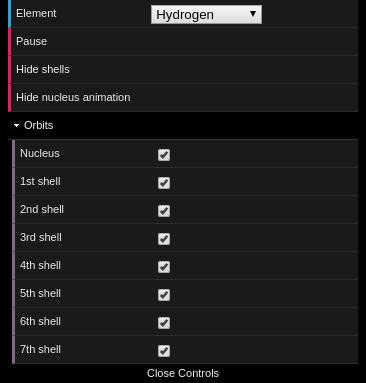
\includegraphics[scale=0.4]{controls.png}
\caption{Controls}
\label{fig:fig4}
\end{figure}

Moreover, it is also possible to select which of the layers to show, what makes easy to see how many electrons are orbiting each layer.

\subsection{Information card}

On the other side of the screen the information of each element is shown, as can be seen in figure \ref{fig:fig6}. All the information is located in a json file and is the base of the application, once it is necessary to calculate the number of spheres of each element as well as the electron shells distribution.

\begin{figure}[!ht]
\centering
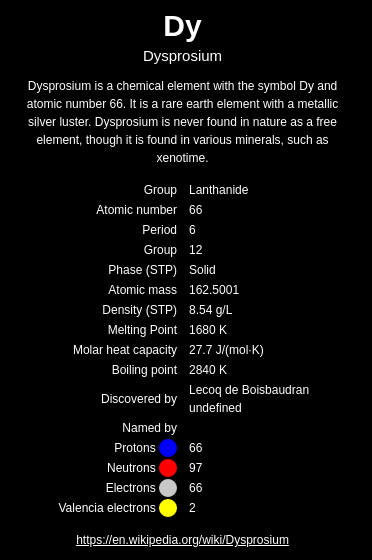
\includegraphics[scale=0.4]{information.png}
\caption{Information sheet}
\label{fig:fig6}
\end{figure}

\subsection{Libraries used}

Below is the list of third-party libraries used for this project.

\begin{itemize}
    \item \textbf{dat.gui.min.js}
    \item \textbf{OrbitControls.js}
    \item \textbf{stats.min.js}
    \item \textbf{three.js}
    \item \textbf{three.min.js}
\end{itemize}

%-------------------------------------------------------------------------------

\section{Conclusion}

Since the beginning, the idea of this project has been to implement an interactive and easy way to see and learn about chemical elements, and it is interesting how much difference it can make in the learning process of a child with basically no effort. This project took me basically one week from start to finish, considering learning WebGL and revising some chemistry lessons.

There was basically one challenge of solving the sphere packing problem, which ended up taking more time that I intended, however the goal was achieved and the final result is very satisfactory. 

%-------------------------------------------------------------------------------

\end{document}